\documentclass{standalone}
\usepackage{tikz}
\usetikzlibrary{arrows.meta}

\begin{document}
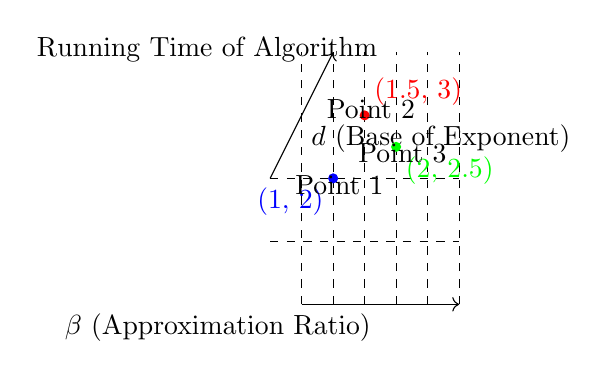
\begin{tikzpicture}[scale=0.8]
    % Define axis limits and ticks
    \def\xmin{0.5}
    \def\xmax{3}
    \def\ymin{2}
    \def\ymax{4}
    
    % Draw axes
    \draw[->] (\xmin, 0) -- node[below left] {$\beta$ (Approximation Ratio)} (\xmax, 0);
    \draw[->] (0, \ymin) -- node[below right] {$d$ (Base of Exponent)} (\xcoord, \ymax);
    
    % Draw grid
    \foreach \x in {\xmin,1,...,\xmax} \draw[dashed] (\x,0) -- (\x,\ymax);
    \foreach \y in {\ymin,1,...,\ymax} \draw[dashed] (0,\y) -- (\xmax,\y);
    
    % Plot points
    \filldraw[blue] (1, 2) circle[radius=2pt] node[anchor=north east] {(1, 2)};
    \filldraw[red] (1.5, 3) circle[radius=2pt] node[anchor=south west] {(1.5, 3)};
    \filldraw[green] (2, 2.5) circle[radius=2pt] node[anchor=north west] {(2, 2.5)};
    
    % Add labels to points
    \node at (1.1, 1.9) {Point 1};
    \node at (1.6, 3.1) {Point 2};
    \node at (2.1, 2.4) {Point 3};
    
    % Add title
    \node[above left] at (2, 3.7) {Running Time of Algorithm $\vcmaxdegthree$};
\end{tikzpicture}
\end{document}